\documentclass{article}
\usepackage{template/iclr2026_conference,times}
\usepackage[T1]{fontenc}
\usepackage[utf8]{inputenc}
\usepackage{microtype,graphicx,booktabs,amsmath,amssymb,array,tabularx,multirow,seqsplit}
\usepackage[dvipsnames,table]{xcolor}
\usepackage{caption,float}
\usepackage{url}
\usepackage[colorlinks=true,linkcolor=MidnightBlue,citecolor=MidnightBlue,urlcolor=MidnightBlue]{hyperref}
\iclrfinalcopy
\urlstyle{same}
\definecolor{paperblue}{HTML}{245C91}
\captionsetup{font=small,labelfont=bf,skip=5pt,justification=raggedright,singlelinecheck=false}
\definecolor{tablewash}{HTML}{EEF4F9}
\renewcommand{\arraystretch}{1.15}
\newcolumntype{Y}{>{\raggedright\arraybackslash}X}
\setlength{\textfloatsep}{12pt}
\setlength{\intextsep}{7pt}
\setlength{\tabcolsep}{5pt}
\newcommand{\sys}{Knolling Bot v2}
\newcommand{\pct}{\%}
\newcommand{\code}[1]{\texttt{\small #1}}
\newcommand{\Hbeta}{H_{\beta}}
\title{\normalfont\LARGE\bfseries Knolling Bot v2:\\Language-Guided Object Arrangement}
\author{Minjae Bang\\Department of Computer Science\\Columbia University}
\hypersetup{pdftitle={Knolling Bot v2: Language-Guided Object Arrangement},pdfauthor={Minjae Bang},pdfsubject={Language-conditioned object arrangement; course research paper}}
\renewenvironment{abstract}{\vspace{4pt}\noindent\textbf{Abstract.}\ }{\par\vspace{3pt}}
\begin{document}
\maketitle
\lhead{}
\rhead{}
\renewcommand{\headrulewidth}{0pt}
\vspace{-12pt}
\begin{figure}[H]
\centering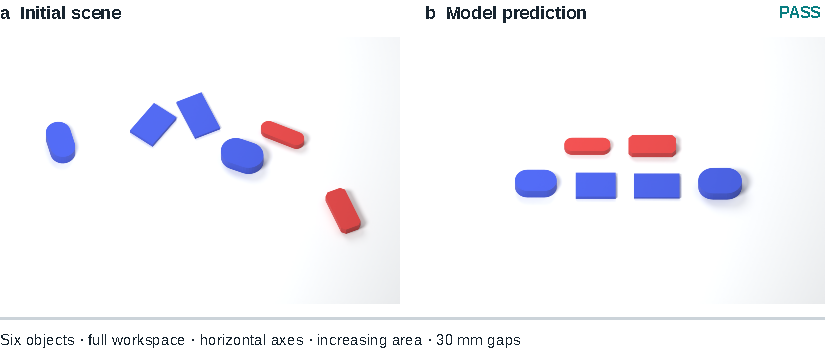
\includegraphics[width=\linewidth]{figures/qualitative_full_annotated.pdf}
\caption{\textbf{Language-guided arrangement.} Matched Blender views of a saved six-object validation prediction preserve original meshes and recorded poses. The instruction specifies horizontal axes, increasing area, and 30\,mm gaps. The model consumes original overhead RGB, not these presentation renders.}
\label{fig:qualitative}
\end{figure}
\vspace{-10pt}
\begin{abstract}
We study language-guided knolling from overhead RGB to planar target poses. Object-centric perception and language-conditioned row/order prediction feed constrained geometric decoding. On 128 sealed families comprising 640 image--instruction pairs, v2 achieves 540/640 strict successes (84.4\%), versus 489/640 (76.4\%) for its predecessor with the same learned base. The paired gain is 8.0 percentage points (family-bootstrap 95\% interval: 4.8--11.6), with no lost successes. Spacing errors affect 71 of 100 remaining failures. The project targets end-to-end learning; the evaluated system uses staged training and explicit rules. A broader joint-training pilot failed. Stable joint learning and physical execution remain open objectives.
\end{abstract}

\section{Introduction}
Knolling organizes objects into aligned, evenly spaced layouts for tasks such as assembly preparation. Visual neatness is insufficient: moving an unselected object, missing a gap, or crossing a region boundary invalidates an instruction. We ask: \emph{How reliably can an RGB-and-language system satisfy all arrangement constraints at once?}

The system handles two to eight objects and full, color-selective, or no-op commands without teacher poses at inference. Its central design separates \emph{discrete structure} (row membership and order) from \emph{metric placement} (coordinates consistent with estimated sizes and gaps). We contribute this integrated pipeline with selective preservation, a family-separated paired evaluation, and analysis of why local improvements can leave complete-task failures unresolved.

\paragraph{Related work.}
Knolling Bot predicts tidy placements sequentially \citep{hu2025knolling}; its graspability extension addresses clutter \citep{hu2023knolling2}. Our ``v2'' denotes this project's separate release. StructFormer uses point clouds for language-guided structure \citep{liu2022structformer}, while Transporter Networks and CLIPort predict manipulation actions \citep{zeng2021transporter,shridhar2022cliport}. Our calibrated RGB-to-layout task measures complete geometric validity; different inputs, tasks, and metrics preclude a direct performance ranking.

\clearpage
\section{Method}
\label{sec:method}
Given overhead RGB $I\in[0,1]^{3\times384\times576}$ and English instruction $t$, the system predicts $\hat P=\{(\hat x_i,\hat y_i,\hat\theta_i)\}_{i=1}^{\hat N}$ in a $0.60\times0.40$\,m workspace. Long axes are $\pi$-periodic. Commands arrange all objects, a named color, or preserve the scene. Preferences specify region, 15/20/30\,mm gaps, color rows, area order, and axis. ``Vertical'' rotates objects; rows still run left to right.

\begin{figure}[H]
\centering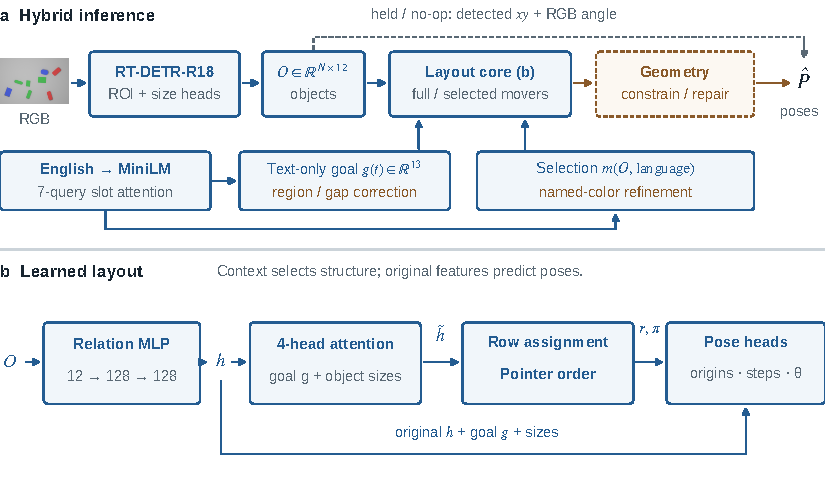
\includegraphics[width=\linewidth]{figures/architecture_main.pdf}
\caption{\textbf{Hybrid inference and the learned layout core.} Contextual features select rows and pointer order; pose heads read original relation features. Blue denotes learned modules and brown explicit rules. The global goal $g$ is text-only; selection $m$ also reads objects. Held/no-op objects bypass layout prediction and retain estimated source poses.}
\label{fig:architecture}
\end{figure}

\paragraph{Perception and language grounding.}
RT-DETR-R18 \citep{zhao2024rtdetr}, from the DETR family \citep{carion2020detr}, supplies queries and physical attributes. Crop-conditioned appearance and size heads refine each detection. Retained objects form 12-dimensional vectors of position, size, angle, color, and shape. MiniLM \citep{wang2020minilm,reimers2020multilingual} supplies text tokens to seven learned goal queries, producing a 13-dimensional global goal. A separate object--language attention branch predicts per-object selection. Explicit English templates correct disagreeing region/gap bins.

\paragraph{Learned structure and constrained coordinates.}
A relation encoder produces features $h_i\in\mathbb R^{128}$. Four-head set attention conditions row assignment $r$ and pointer order $\pi$ on the goal and object sizes; pose heads retain the original $h_i$. The initial search ranks structures by row/order log-probabilities and checks at most eight candidates. The full route enforces predicted-area order. For feasible aligned neighbors, the geometry follows
\begin{equation}\label{eq:mainspacing}
 \hat x_{j+1}-\hat x_j=\tfrac12(\hat w_j+\hat w_{j+1})+d,\qquad |d-\delta|\leq2\,\mathrm{mm},
\end{equation}
where $\hat w_j$ is the rotated horizontal extent and $\delta$ the requested gap. Row heights similarly govern vertical spacing. Estimated dimensions determine metric placement, while the neural selector chooses structure. Conditional repair ranks alternative rows by row probabilities; an unsuccessful bounded repair retains the original prediction. Feasibility is not guaranteed.

\paragraph{Selective preservation.}
Partial placement selects the named color and searches translations around held objects. Held/no-op centers use detections; angles use RGB silhouette principal-component analysis with a learned fallback. Preservation therefore requires accurate perception. Appendix~\ref{app:implementation} specifies routing and search bounds.

\clearpage
\section{Data, Training, and Evaluation}
\label{sec:protocol}
\paragraph{Synthetic corpus.}
The corpus contains 4,000 geometry families and 20,000 image--instruction pairs. Five commands share each RGB image: three full arrangements, one color-selective task, and one no-op. These controlled contrasts vary instructions while holding the scene fixed. Procedural boxes, chamfers, and capsules have red, green, or blue appearances. A geometric teacher generates layouts; an independent validator checks acceptance. Images use Blender Cycles. The split is 3,200/400/400 families, or 16,000/2,000/2,000 pairs, for train/validation/test. Family separation prevents identical source images from crossing pools. Corpus size is not the exposure of every training stage.

\paragraph{Staged optimization.}
Perception and arrangement bases are trained separately. Subsequent relation stages use a 791-pair train manifest and 94-pair validation manifest. A size-residual stage uses source-dimension supervision. Restricted joint fine-tuning then updates only the size residual and selected row-coordinate parameters; perception, language, goal, relation, row assignment, order, and angle heads remain frozen. Refined sizes are detached before the pose computation, so pose loss does not train perception. The selector trains row and pointer cross-entropies on 5,085 usable full-arrangement pairs from 5,376 eligible pairs (1,792 train families); 291 pairs fail detection-count or association checks. Eight epochs are recorded, with epoch 1 selected using 1,200 full validation pairs. Losses, hyperparameters, gradient boundaries, and historical diagnostics appear in Appendix~\ref{app:training}.

A broader joint-training pilot was attempted but rejected after collapse: at update 200, success fell from 2/38 to 0/38 on development and from 24/152 to 1/152 on validation. This observation motivated retaining the stable staged system. It is one unsuccessful configuration, not evidence that end-to-end training is impossible.

\paragraph{Sealed release comparison.}
The final evaluation uses a later, separately generated set of 128 families and 640 pairs. Family IDs, RGB hashes, and asset-family IDs are disjoint from the 20,000-pair corpus. Its objects use the development asset pool not rendered in the 20,000-pair corpus, within the same procedural shape/color vocabulary. The recorded modes are 384 full, 127 partial, and 129 no-op pairs. Both releases were scored on these same records with the same evaluator and threshold. Neither this set nor the official 2,000-pair test split was used to select v2 checkpoints or thresholds. This paper reaggregates the stored sealed scores; it does not rerun inference or select a new model on them.

\paragraph{Strict complete-scene success.}
A count mismatch immediately fails. Otherwise Hungarian matching associates predicted source objects with true identities; each association must meet a 10\,mm center-error limit and envelope IoU $\geq0.5$. Target poses are then checked using true object geometry. Every applicable constraint must pass: selection/preservation, requested region, axis, row alignment, gaps, color grouping, size order, collision, clearance, and boundary. The score is the mean binary scene outcome,
\begin{equation}
 S=\frac{1}{M}\sum_{s=1}^{M}\mathbf{1}\{\hat N_s=N_s\ \land\ \text{identity and task checks pass}\}.
\end{equation}
This measures valid instruction fulfillment, not exact reproduction of one teacher layout. A different valid arrangement can pass. It does not measure grasp success, trajectory safety, visual aesthetics, or physical execution.

\begin{table}[H]
\centering\small
\caption{Prediction-scoring thresholds. Dataset acceptance has a separate contract; in particular, stored locked poses must copy the source exactly.}
\label{tab:tolerances}
\begin{tabular*}{\linewidth}{@{}l@{\extracolsep{\fill}}l@{}}\toprule
\textbf{Check} & \textbf{Threshold / requirement} \\\midrule
Held position / long-axis angle & $\leq1$\,mm / $\leq1^\circ$ deviation \\
Requested axis / row alignment & $\leq2^\circ$ / $\leq2$\,mm deviation \\
Horizontal / vertical gap & $\leq2$\,mm from requested gap \\
Object clearance / table margin & At least 10\,mm (0.1\,mm numerical tolerance) \\
Size order & At most 5\% area inversion \\\bottomrule
\end{tabular*}
\end{table}

\clearpage
\section{Results and Analysis}
\label{sec:results}
\paragraph{A paired improvement with the learned base fixed.}
Table~\ref{tab:main} compares releases with unchanged learned architecture and checkpoint-loading paths. V2 adds 10\,mm duplicate suppression, sentence-consistent region/gap choices, stricter named-color selection, and feasibility-gated row/color repair. It evaluates this inference bundle over the same learned base, rather than additional training or isolated component effects.

\begin{table}[H]
\centering
\caption{Strict target-layout success on the independent 640-pair set. Counts are successful scenes / evaluated scenes. Gains are paired percentage-point differences; neither system executes a robot.}
\label{tab:main}
\begin{tabularx}{\linewidth}{Yrrr}\toprule
\textbf{Task} & \textbf{v1.0.0} & \textbf{v2.0.0} & \textbf{Gain (pp)} \\\midrule
Full & 287/384 (74.7\%) & 311/384 (81.0\%) & +6.3 \\
Partial & 84/127 (66.1\%) & 104/127 (81.9\%) & +15.7 \\
No-op & 118/129 (91.5\%) & 125/129 (96.9\%) & +5.4 \\\midrule
\rowcolor{tablewash} Overall & 489/640 (76.4\%) & \textbf{540/640 (84.4\%)} & \textbf{+8.0} \\\bottomrule
\end{tabularx}
\end{table}

V2 retains all 489 v1 successes and gains 51: 24 full, 20 partial, and 7 no-op scenes. Failures fall from 151 to 100 (33.8\% relative reduction). Five instructions share each image, so uncertainty resamples paired \emph{families}. Across 10,000 bootstrap resamples, the 95\% interval is +4.8 to +11.6 points. Twenty-nine families improve, 99 tie, and none worsen. This interval covers evaluation-family variation conditional on the frozen systems, not training-seed uncertainty or real-world domain shift.

\begin{figure}[H]
\centering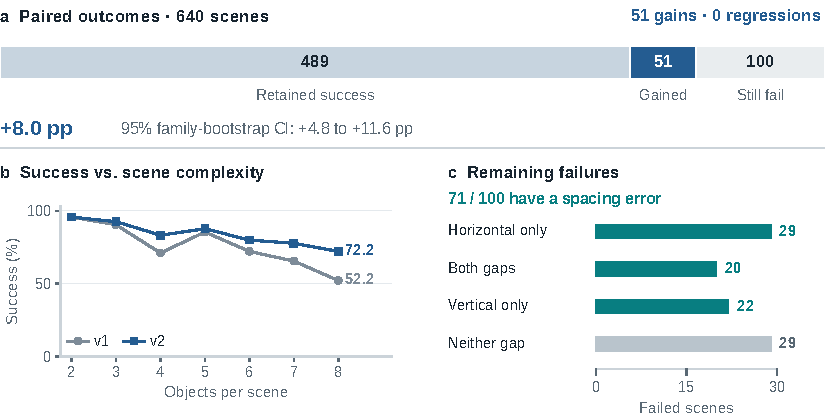
\includegraphics[width=\linewidth]{figures/holdout_diagnostics.pdf}
\caption{\textbf{Paired gains and remaining difficulty.} (a) V2 retains all 489 baseline successes and gains 51; uncertainty resamples 128 paired families. (b) Success generally decreases with object count (90--95 pairs per bin). (c) Four mutually exclusive gap categories partition the 100 v2 failures. Other error types may coexist; Appendix~\ref{app:statistics} lists raw, overlapping tags.}
\label{fig:results}
\end{figure}

\paragraph{What improved, and what remains difficult?}
Partial tasks show the largest gain. Count failures fall from 45 to 5, and region failures from 17 to 4. These changes are consistent with the added rules, but do not identify their individual causal contributions. Eight-object success rises from 47/90 to 65/90 (52.2\% to 72.2\%), remaining below the two-object bin (91/95 for both).

Spacing dominates: 49 horizontal-gap and 42 vertical-gap failures overlap in 20 scenes, affecting 71/100 failures. Other tags are 11 size-order, 7 clearance, 5 count, 4 region, and 4 preservation errors. Internal feasibility uses \emph{predicted} dimensions; scoring uses true rectangles. Internally valid geometry can therefore miss the gap threshold---a plausible mechanism, whose frequency the tags alone cannot establish.

\clearpage
\section{Interpreting Predicted Arrangements}
\label{sec:discussion}
\begin{figure}[H]
\centering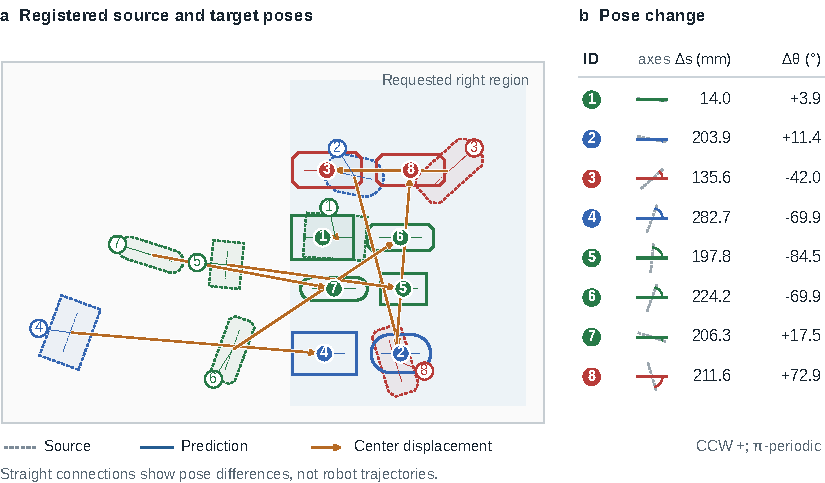
\includegraphics[width=\linewidth]{figures/motion_correspondence.pdf}
\caption{Object-level motion in the eight-object validation example. Dashed footprints mark recorded source poses and solid outlines mark saved predictions, in a common world frame. Matched IDs and straight center-displacement arrows establish correspondence. The ledger shows translations and signed, $180^\circ$-periodic long-axis rotations; its glyphs compare source and target axes. Arrows are not robot trajectories.}
\label{fig:motion}
\end{figure}

\paragraph{Valid tasks require more than tidy appearance.}
Figures~\ref{fig:modes}--\ref{fig:diagnostics} locate the violations in a separate three-command example. Its full-layout row gap exceeds the allowed upper limit by 0.657\,mm. The partial-layout clearance misses the tolerance-adjusted minimum by only 3.9\,$\mu$m: a borderline score failure, not a visible collision. This distinction exposes sensitivity to geometric estimates and scoring thresholds; it does not establish real-world positioning precision. Complete-scene validity also need not track local selector accuracy (Appendix~\ref{app:training}).

\paragraph{End-to-end scope.}
RGB and English produce poses without teacher information at inference. Staged losses, discrete selection, template correction, image-based angle estimation, and geometry remain essential; successful joint training is unproven. No real-image, paraphrase, severe-occlusion, or physical evaluation is available. Static clearance is not a safe manipulation sequence.

\paragraph{Evidence limits.}
Evaluation covers a calibrated synthetic domain with three colors/shape types and at most eight objects, using one learned base without factorial ablation or multiple seeds. The 0.137\,s median inference time is not a deployment benchmark. Missing historical trainers and undistributed checkpoints prevent exact retraining; the package reproduces the paper's analysis and visualization.

\section{Conclusion}
\sys\ achieves 84.4\% strict scene success, improving by 8.0 points over its predecessor on a sealed, family-separated set. The results support a staged hybrid system where identity, instruction consistency, and geometry jointly determine success. Next steps are dimension-sensitive spacing, controlled ablations, stable joint optimization, and physical validation.

\clearpage
\begingroup
\raggedright
\bibliography{references}
\bibliographystyle{template/iclr2026_conference}
\endgroup
\clearpage
\appendix
\section{Implementation Details}
\label{app:implementation}
\paragraph{Coordinate and object contract.}
The origin is the workspace's bottom-left corner; positions are metres and angles are radians counterclockwise from $+x$, modulo $\pi$. Image coordinates are $p_x=576x/0.6-0.5$, $p_y=384(1-y/0.4)-0.5$. Each object is encoded as
\begin{equation}
 o_i=[x_i/0.6,\ y_i/0.4,\ a_i/0.6,\ b_i/0.4,\ \cos(2\theta_i),\ \sin(2\theta_i),\ c_i^{(1:3)},\ q_i^{(1:3)}],
\end{equation}
where $a_i,b_i$ are predicted major/minor dimensions and $c_i,q_i$ are color/shape probabilities. Inference accepts one to eight detections; evaluated scenes contain two to eight objects.

\begin{table}[H]
\centering\small
\caption{Implementation dimensions and decisions in the adopted inference path.}
\begin{tabularx}{\linewidth}{@{}lY@{}}\toprule
\textbf{Component} & \textbf{Implementation} \\\midrule
Perception & RT-DETR-R18; 3 decoder layers; 300 width-256 queries; internal $640\times640$ input. \\
Appearance adapter & $16\times16$ predicted-box crop; CNN $3\to16\to32$; query/crop head $288\to128\to10$. \\
Size residual & $8\times8$ crop; 16-channel CNN feature + query; MLP $272\to64\to2$; dimension floor $10^{-4}$\,m. \\
Language & MiniLM tokens $384\to128$; 7 goal queries; four-head text attention; feed-forward $128\to512\to128$. \\
Goal / selection & Text-only goal: keep (1), axis (2), region (3), gap (3), grouping (2), order (2). Separate selection: object $12\to128$, self-/language attention, head $128\to1$. \\
Relation / context & MLP $12\to128\to128$; one width-128, four-head set-attention block for structure. \\
Structure & Row MLP $141\to128\to8$; pointer query $269\to128\to128$, masked dot-product selection. \\
Pose heads & Row origin $417\to128\to2$; X step $3\to32\to1$; angle $141\to128\to2$, half-atan2 decoding. \\
Filtering / search & Foreground threshold 0.5; duplicate-center radius 10\,mm; at most eight checked candidates per search. \\\bottomrule
\end{tabularx}
\end{table}

For keep probability $k$ and attribute distributions $p_a,p_r,p_\delta,p_c,p_s$, the goal is $g=[k,(1-k)p_a,(1-k)p_r,(1-k)p_\delta,(1-k)p_c,(1-k)p_s]$. Tokens $z_i=h_i+W_g g+W_s s_i$ are normalized before self-attention is added to $h_i$; a null key handles padding. Context guides row/order selection; pose heads use original $h_i$. Rows and pointer prefixes are predicted at inference, with teacher forcing only in training. Each row shares its neural origin's $y$ coordinate; positive X steps use $\operatorname{softplus}(\operatorname{MLP}([w_{j-1},w_j,\delta]))$.

The ideal axis-aligned spacing is
\begin{equation}
 x_{j+1}-x_j=\tfrac12(w_j+w_{j+1})+\delta,\qquad
 y_r-y_{r+1}=\tfrac12(H_r+H_{r+1})+\delta_r,
\label{eq:spacing}
\end{equation}
where $w_j$ is horizontal extent, $H_r$ the maximum row height, and $\delta_r=2\delta$ between color bands ($\delta$ otherwise). The implemented decoder uses rotated rectangles and $\pm2$\,mm gap bands rather than exact equalities. Regions $(x_{\min},y_{\min},x_{\max},y_{\max})$ are full $(.02,.02,.58,.38)$, left $(.02,.02,.28,.38)$, and right $(.32,.02,.58,.38)$; a fitting layout may shift 1\,mm inward.

The initial search ranks candidates by row and pointer scores; repair/color-split searches use row scores. Enumeration may consider more partitions before truncation. Explicit area-order enforcement applies on the full route and in invoked repair, not universally on the partial route. Exhausted repair retains the original prediction: neither feasibility nor global optimality is guaranteed. Preservation details appear in Appendix~\ref{app:qualitative}.

\clearpage
\section{Training Evidence and Optimization}
\label{app:training}
\begin{table}[H]
\centering\small
\caption{Recorded training stages. These are stage-specific exposures, not repeated full-corpus training. The official test and independent final holdout are excluded.}
\begin{tabularx}{\linewidth}{@{}lY@{}}\toprule
\textbf{Stage} & \textbf{Evidence and scope} \\\midrule
Base integration & Separate perception and arrangement checkpoints at updates 2,400 and 6,000, respectively. \\
Relation stages & 791 training and 94 validation pairs; seed 1203. The final pipeline reuses only the relation hidden encoder. \\
Size residual & 3,200 train source families, divided into 2,560 fit / 640 development; batch 8; learning rate $10^{-3}$; selected update 200. \\
Restricted joint & Official train families split 4/5 fit, 1/5 development; batch 4; AdamW, learning rate $10^{-5}$, weight decay 0; 30 updates, 120 attempted presentations, 6 excluded. \\
Set selector & 1,792 eligible train families, 5,376 full pairs, 5,085 usable; 249 association and 42 count exclusions; 8 epochs / 1,272 updates; initial learning rate $10^{-4}$; selected epoch 1. \\
Broad joint pilot & Seed 1203; batch 2; encoder / goal / hidden / row learning rates $10^{-6}/10^{-5}/10^{-5}/10^{-4}$; stopped at update 200 after collapse; not adopted. \\\bottomrule
\end{tabularx}
\end{table}

\paragraph{Losses and gradient boundaries.}
Write the SmoothL1 penalty as $H_\beta(e)=e^2/(2\beta)$ if $|e|<\beta$, and $|e|-\beta/2$ otherwise. Let $d_\pi(\alpha,\beta)=((\alpha-\beta+\pi/2)\bmod\pi)-\pi/2$. The size residual minimizes
\begin{equation}
 \mathcal L_{\mathrm{size}}=\operatorname{mean}_{i\in M,k\in\{a,b\}}H_{.001}(\hat s_{ik}-s^*_{ik}).
\end{equation}
$M$ denotes matched objects. Matching uses true source centers only during supervision; detector outputs and predicted crop boxes are detached. The selector's recorded objective is row cross-entropy plus teacher-forced pointer cross-entropy,
\begin{equation}
 \mathcal L_{\mathrm{select}}=\operatorname{CE}(R,r^*)+\operatorname{CE}(O,\pi^*),
\end{equation}
with invalid/padded targets ignored. The recorded total equals these two losses; no extra color regularizer is assumed.

In restricted joint fine-tuning, let $G$ contain reference predictions within 2\,mm position error and $3^\circ$ angle error, and $F$ contain the other valid objects. The recorded objective is
\begin{align}
\mathcal L_{\mathrm{joint}}={}&\mathcal L_{\mathrm{size}}
+\operatorname{mean}_{i\in F,k\in\{x,y\}}H_{.010}(\hat p_{ik}-p^*_{ik})
+\operatorname{mean}_{i\in F}|d_\pi(\hat\theta_i,\theta_i^*)|\nonumber\\
&+\operatorname{mean}_{i\in G,k\in\{x,y\}}H_{.001}(\hat p_{ik}-p^{\mathrm{ref}}_{ik}).
\end{align}
Empty terms are zero. Only the size residual, horizontal step head, and final row-origin layer update. Refined sizes are stop-gradient before the pose forward pass; perception, language, goal, relation, structure, and angle heads are frozen. Consequently the angular term contributes to the loss value but cannot update the frozen angle head. This is a restricted multi-head update, not a differentiable joint objective through the entire system.

\paragraph{Development evidence and its limits.}
The saved 152-scene full-arrangement diagnostic improves from 24 to 42 successes after size refinement and from 42 to 54 after restricted joint tuning. Size refinement reduces median major-dimension error from 1.419 to 0.790\,mm (796 matched objects), while restricted joint tuning reduces median vertical-gap error from 2.015 to 1.588\,mm. These are recorded development stages with evolving code and selection gates, not independent final-test ablations. In contrast, the broader joint pilot falls from 2/38 to 0/38 development successes and from 24/152 to 1/152 validation successes at update 200; the best checkpoint remains update 0. A historical 260-scene diagnostic overlapped earlier fitting data and is excluded from claims of independent generalization.

\clearpage
\subsection{Selector Learning Curve}
\begin{figure}[H]
\centering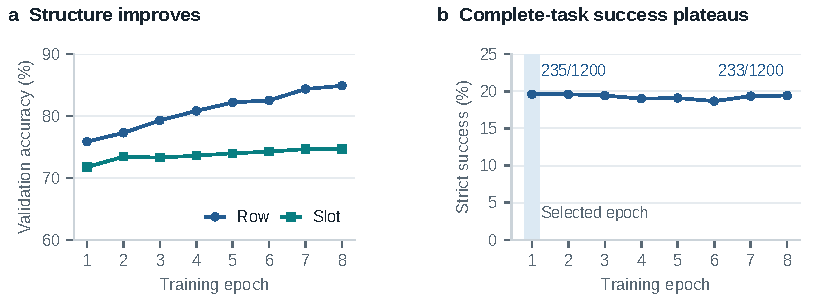
\includegraphics[width=\linewidth]{figures/selector_training.pdf}
\caption{Historical selector-stage validation on 1,200 full-arrangement pairs, before the final inference refinements. Row and slot accuracy improve, but complete-scene success plateaus. This is a component-training diagnostic, not the final independent evaluation. Values are read from the saved eight-epoch curve.}
\label{fig:training}
\end{figure}

The baseline succeeds on 222/1200 pairs. Epoch 1 reaches 235/1200, with row/slot accuracy of 75.86\%/71.77\% (baseline: 68.52\%/61.87\%). Mixed-color-row tags fall from 234 to 22. At epoch 8, row/slot accuracy reaches 84.88\%/74.68\%, but success is 233/1200. Improved structure need not remove a scene's last violation.

\section{Data and Statistical Details}
\label{app:statistics}
Scene and asset seeds are 120912 and 120913, respectively. Major dimensions span 40--80\,mm, minor dimensions 25--50\,mm, and heights 5--20\,mm on a 1\,mm grid, with aspect ratio $\geq1.3$. The corpus uses \code{continuous\_rows\_v3} teacher layouts and \code{english\_rows\_v1} instructions. For family $i$, bucket $\lfloor i/20\rfloor\bmod10$ assigns 0--7 to train, 8 to validation, and 9 to test. These pools also use mutually disjoint sets of 64 asset families each. Source clearance/margin is 12\,mm; accepted targets require 10\,mm and exact source copies for locked poses. Independent validation checks targets. Dataset RGB rendering used Blender 5.1.0, Cycles CPU, and 32 samples; PNG bytes may vary across environments.

The separate final set uses scene seed 20261112, registry seed 120913, and development assets. Its 128 families/640 pairs share no geometry-family IDs, RGB hashes, or asset-family IDs with the corpus. This tests new instances within the procedural domain. Mode labels follow teacher outcomes: already-satisfied color-selective commands become no-op. Actual mode counts determine denominators.

\paragraph{Paired bootstrap.}
Define $d_f=\frac15\sum_{j=1}^{5}(Y^{v2}_{fj}-Y^{v1}_{fj})$. Resample 128 families with replacement and compute $100\operatorname{mean}_f d_f$, preserving five paired outcomes per family. Python's local random generator (seed 20261112) produces 10,000 replicates; sorted indices 250 and 9749 give 4.84375 and 11.5625 points. The observed gain is 7.96875 points. Paired counts are 489 both-pass, 51 v2-only, 0 v1-only, and 100 both-fail. This reaggregation does not rerun model evaluation.

\begin{table}[H]
\centering\small
\caption{All nonzero error tags across either release. Tags overlap; horizontal and vertical gaps coincide in 20 v2 scenes.}
\begin{tabular*}{\linewidth}{@{}l@{\extracolsep{\fill}}rrlrr@{}}\toprule
\textbf{Error} & \textbf{v1} & \textbf{v2} & \textbf{Error} & \textbf{v1} & \textbf{v2} \\\midrule
Horizontal gap & 51 & 49 & Clearance & 9 & 7 \\
Vertical gap & 48 & 42 & Keep pose & 9 & 4 \\
Object count & 45 & 5 & Mixed-color row & 2 & 0 \\
Requested region & 17 & 4 & Collision & 1 & 0 \\
Size order & 13 & 11 & Boundary & 1 & 0 \\\bottomrule
\end{tabular*}
\end{table}

\clearpage
\section{Command Dependence and Object Correspondence}
\label{app:qualitative}
\begin{figure}[H]
\centering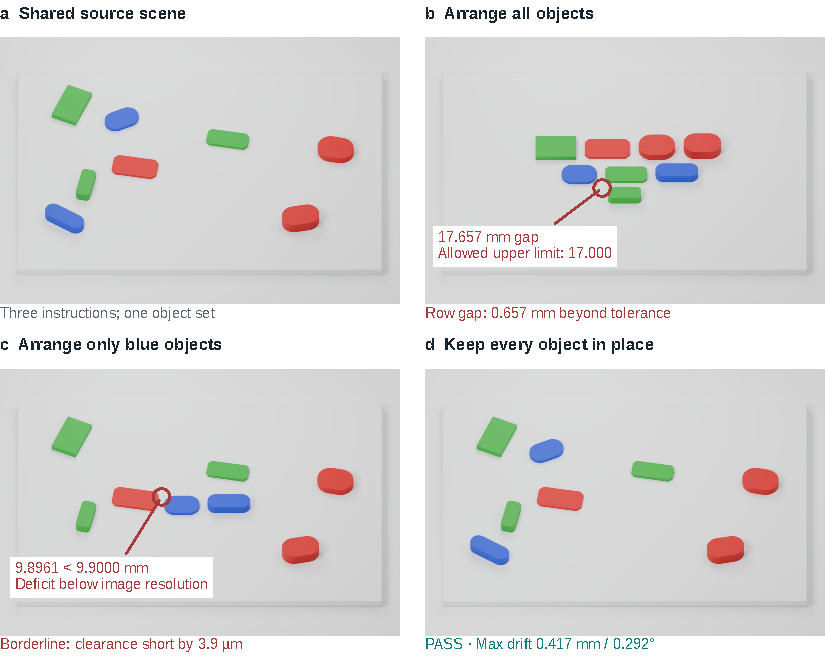
\includegraphics[width=\linewidth]{figures/qualitative_modes.pdf}
\caption{One validation scene under three commands, rendered with the same Blender camera and lighting. (b) fails because a row gap is 0.657\,mm past its upper limit. (c) fails clearance by 3.9\,$\mu$m, a deficit this print cannot resolve. (d) passes, with at most 0.42\,mm and 0.29$^\circ$ of drift from the source. Figure~\ref{fig:diagnostics} measures (b) and (c) on overhead crops.}
\label{fig:modes}
\end{figure}

\paragraph{Preservation implementation.}
For an unambiguous named color, partial mode replaces the moving set with those objects. Held objects constrain a static clearance search that translates the moving block on a 5\,mm grid within $\pm120$\,mm. Held/no-op angles use silhouette PCA on connected components in a local $\pm80$\,mm image window, with chroma threshold $25/255$ and at least 40 pixels. If PCA is unavailable, a direction head supplies the angle; without its checkpoint, the base detector angle is retained. This is static placement, not grasp or trajectory planning.

\paragraph{Pose-change notation.}
Figure~\ref{fig:motion} measures $d_i=1000\|\hat p_i-p_i^{\mathrm{src}}\|_2$ in millimeters and
\begin{equation}
\Delta\theta_i=\frac{180}{\pi}\left[\left(\hat\theta_i-\theta_i^{\mathrm{src}}+\frac\pi2\right)\bmod\pi-\frac\pi2\right].
\end{equation}
IDs match the saved scene objects. Source poses are original scene-record poses, and targets are stored model predictions. World-plane vectors and orientation glyphs describe pose differences only; they do not imply a collision-free manipulation path or an executed robot motion.

\paragraph{Example provenance.}
The smoke script chose the first supported example of each mode from family \code{expanded\_09aa3f57968449ce8a09f291}, with suffixes \code{\_0}, \code{\_2}, and \code{\_3}. The full and partial commands request horizontal axes and 15\,mm gaps; partial selects blue objects. No-op maximum drift is 0.417\,mm and $0.292^\circ$. The six-object opening example is \code{expanded\_e2ee7a75ae3a34826b36d71f\_0}; the eight-object motion example is \code{expanded\_717287879ce16878c5558650\_4}. These selected validation records lack per-record checkpoint digests and illustrate behavior, not a second benchmark. The older ten-image v1 gallery is not used as v2 evidence.

\clearpage
\section{Failure Margins and Rendering Fidelity}
\label{app:failure}
\begin{figure}[H]
\centering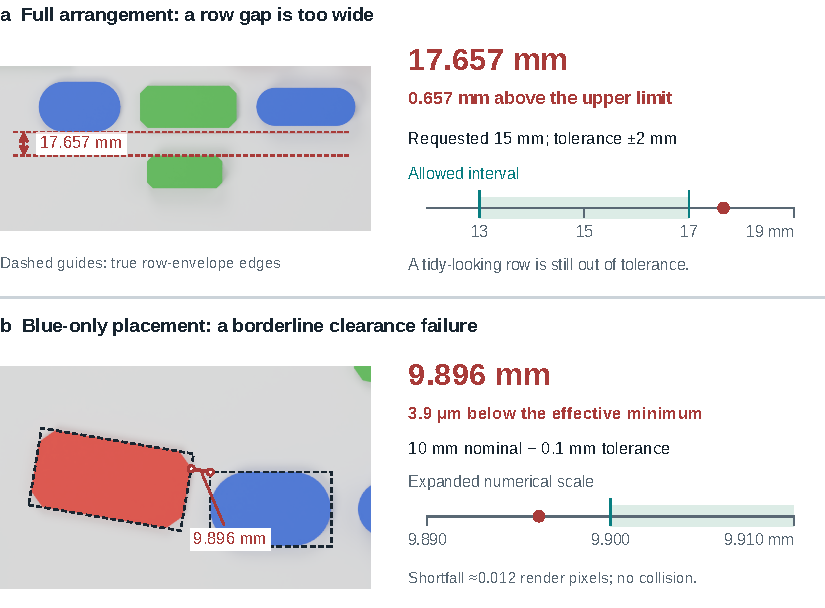
\includegraphics[width=\linewidth]{figures/failure_explanation.pdf}
\caption{Measured violations, not just failure labels. Real Blender closeups mark the evaluated bounding envelopes; the adjacent rulers compare each measured value with its permitted interval. The row gap exceeds 17.000\,mm by 0.657\,mm. Clearance falls about 3.9\,$\mu$m below 9.900\,mm, after the evaluator's 0.1\,mm numerical tolerance. Ruler scales differ and are labeled explicitly.}
\label{fig:diagnostics}
\end{figure}

\paragraph{Why the borderline example matters.}
The partial result is not evidence of a visually poor arrangement or a physical collision. Its failure is a precise consequence of the synthetic evaluator's envelope-distance threshold. True mesh silhouettes and oriented bounding rectangles differ, especially for capsules and chamfers; the annotated quantity is rectangle-to-rectangle clearance. This example motivates distinguishing failure severity and scoring margins from a binary success rate. It supplies no estimate of how frequently such near-threshold cases occur across the holdout.

\paragraph{Pose and geometry fidelity.}
Every presentation image renders a preserved scene record. Meshes extrude the project's original footprint polygons to their recorded heights, retaining identity, color, dimensions and source/predicted pose. No layout is adjusted for composition. Before/after views share orthographic camera, illumination, materials, background, and image quality. Blender 5.1.0 uses Cycles CPU, $1920\times1280$ resolution, denoising and adaptive sampling with a 128-sample maximum. Overhead closeups use the same materials and lighting with a calibrated camera.

The original $576\times384$ RGB images remain the actual inference inputs (one appears in Figure~\ref{fig:architecture}); presentation renders are generated only afterward. Input/output hashes, object transforms, camera settings, editable Blender scenes and scripts are included. An independent check reopens every saved scene and compares all object transforms and mesh vertices with the source records. The only residual differences are float32 storage quantization, below $10^{-7}$ in the corresponding meter/radian coordinates. No additional model inference or training is performed.

\clearpage
\section{Reproducibility and Evidence Package}
\label{app:reproducibility}
The analysis compares v1.0.0 (\code{26dca53}) and v2.0.0 (\code{593bd5d}); the release-candidate measurement was carried forward without changing inference. Manuscript preparation used checkout \code{535f14f}. The adopted entry points are \code{load\_adopted} in the end-to-end scorer and \code{poses\_from\_detection} in \code{size\_refinement.py}. Source-identity matching minimizes a Hungarian cost incorporating confidence, source position, size, and angle. Each match must additionally satisfy center distance $\leq10$\,mm and oriented-envelope IoU $\geq0.5$; otherwise the scene fails with \code{source\_identity}. Target poses then undergo the independent semantic and geometry checks.

The model runtime uses Python 3.12, PyTorch 2.9.1, torchvision 0.24.1, and transformers 4.57.3. The text backbone is \code{paraphrase-multilingual-MiniLM-L12-v2}; pretrained snapshots are pinned in \code{configs/pretrained\_rtdetr.json}. Reloading requires local base/parent checkpoints, relation, joint row/size and selector weights, selection/direction heads, and pretrained caches. The source repository does not distribute these weights or datasets, and the historical selector trainer and independent-set generator are absent. The package below supports reproduction of the \emph{paper's analysis and figures}, rather than claiming full training reproduction.

\paragraph{Version-controlled change.}
The v1.0.0--v2.0.0 changes are inference refinements: duplicate suppression, sentence-consistent region/gap choices, exact named-color mover replacement, infeasible-row repair, and feasible color-row splitting. Architecture, loading paths, set attention, size residual, constraint search, and PCA correction are shared. Individual effects remain unmeasured.

\begin{table}[H]
\centering\small
\caption{Manuscript evidence package. Paths are relative to the submission root. Full SHA-256 values and original paths are preserved in the audit manifests.}
\label{tab:package}
\begin{tabularx}{\linewidth}{@{}lY@{}}\toprule
\textbf{Artifact} & \textbf{Purpose} \\\midrule
\code{audit/evidence/v1\_holdout.jsonl} & Frozen baseline scores; SHA-256 prefix \code{89b3ee1cbc24}. \\
\code{audit/evidence/v2\_holdout.jsonl} & Frozen v2 scores; prefix \code{209df3c1b12c}. \\
\code{audit/verified\_results.json} & Recomputed counts, breakdowns, paired gain and family bootstrap. \\
\code{scripts/audit\_results.py} & Statistical reaggregation without model inference. \\
\code{scripts/make\_figures.py} & Figure rebuild entry point; calls the publication compositor. \\
\code{scripts/render\_publication.py} & Blender source for matched views at saved poses. \\
\code{renders/} & High-resolution PNGs, editable Blender scenes, and pose/camera metadata. \\
\code{audit/evidence/} & Training summaries, qualitative poses, RGB and rendered prediction. \\
\code{audit/method\_audit.md} & Claim-to-code references and gradient boundaries. \\
\code{audit/results\_audit.md} & Claim-to-record references and dataset integrity. \\
\code{template/upstream.json} & Official ICLR template source and exact hashes. \\\bottomrule
\end{tabularx}
\end{table}

\paragraph{Compute scope.}
The selector stage records 1,719 GPU-seconds, not the total project compute. Saved timing gives median 131.5/137.2\,ms and mean 169.2/197.5\,ms for v1/v2. Hardware, warmup, and serving conditions are not controlled sufficiently for a throughput claim. No total training budget, deployment cost, or physical cycle time is established.

\paragraph{Rebuilding.}
The README provides commands and dependency pins. The analysis scripts in Table~\ref{tab:package} reconstruct the statistics and seven figures. Running \code{latexmk -pdf main.tex} compiles the manuscript. All figure PDFs are included, so compilation alone requires neither Python nor a GPU, checkpoints, or the original datasets.

\paragraph{Assistance disclosure.}
Codex assisted with repository and record inspection, primary-source literature discovery, drafting, figure scripting, and LaTeX typesetting. Experimental outcomes come from saved project records. Manuscript preparation performed statistical reaggregation and Blender visualization at fixed saved poses, without generating additional model predictions or training results.

\end{document}
